% answers.tex —— 1977 年·江苏徐州市、徐州地区初试卷 · 参考答案与详细解析片段
% 由 tools/generate_projects.py 依来源总账自 1977/1977_数学真题_江苏徐州市,徐州地区初试_试题.md + 1977/1977_数学真题_江苏徐州市,徐州地区初试_解析正文.md + 1977/1977_数学真题_江苏徐州市,徐州地区初试_答案要点.md 生成，勿手改（改源 MD 后重跑）


\begin{gktip}
固定源 PDF 为初试（预选）卷编排本（原书页码 241—242），只有题面，未附解答。下文各题均为编者独立推导；原卷中文数字题号（一、二、……、十）已按本库规范转写为阿拉伯数字；第 6、7 题示意图按源卷重绘，第 9（2）略图为编者按题意补绘。原卷记号 $\operatorname{tg}$ 在推导中按现行记号写作 $\tan$。
\end{gktip}

\begin{answer}
\gksolhead{1}{}

\textbf{题目}（8 分）：

\Needspace{5\baselineskip}
计算：

\nopagebreak[4]
\[
(-16)\div\left(-2\frac{2}{3}\right)^2+\left(\frac{1}{3}\right)^{-2}\times\left(\frac{3}{8}\right)^0-\left(\frac{9}{16}\right)^{\frac{1}{2}}.
\]

\Needspace{4\baselineskip}
\textbf{解析}

\Needspace{5\baselineskip}
逐项计算：

\nopagebreak[4]
\[
\left(-2\frac{2}{3}\right)^2=\left(-\frac{8}{3}\right)^2=\frac{64}{9},\qquad
\left(\frac{1}{3}\right)^{-2}=9,\qquad
\left(\frac{3}{8}\right)^0=1,\qquad
\left(\frac{9}{16}\right)^{\frac{1}{2}}=\frac{3}{4}.
\]

\Needspace{5\baselineskip}
于是

\nopagebreak[4]
\[
(-16)\div\frac{64}{9}+9\times1-\frac{3}{4}
=-16\times\frac{9}{4}+9-\frac{3}{4}
=-\frac{9}{4}+9-\frac{3}{4}
=\frac{-9-3}{4}+9
=-3+9=6.
\]

\gkanswer{答案：$6$。}

\end{answer}
\begin{answer}
\gksolhead{2}{}

\textbf{题目}（8 分）：

（1） 把 $\dfrac{1}{\sqrt{3}-2}$ 的分母有理化；

（2） 已知 $x=\sqrt{2}+1$，求 $x^2-2x+1$ 的值。

\Needspace{4\baselineskip}
\textbf{解析}

\gksubpart{（1）}

\Needspace{5\baselineskip}
分母乘其有理化因式 $(\sqrt{3}+2)$：

\nopagebreak[4]
\[
\frac{1}{\sqrt{3}-2}
=\frac{\sqrt{3}+2}{(\sqrt{3}-2)(\sqrt{3}+2)}
=\frac{\sqrt{3}+2}{3-4}
=-(\sqrt{3}+2).
\]

\gksubpart{（2）}

\nopagebreak[4]
\[
x^2-2x+1=(x-1)^2.
\]

\Needspace{5\baselineskip}
由 $x=\sqrt{2}+1$ 得 $x-1=\sqrt{2}$，故

\nopagebreak[4]
\[
(x-1)^2=(\sqrt{2})^2=2.
\]

\gkanswer{答案（1）：$-(\sqrt{3}+2)$。}

\gkanswer{答案（2）：$2$。}

\end{answer}
\begin{answer}
\gksolhead{3}{}

\textbf{题目}（8 分）：

求下列三角函数值：

（1） $\cos150^\circ$；

（2） $\operatorname{tg}\left(-\dfrac{\pi}{6}\right)$。

\Needspace{4\baselineskip}
\textbf{解析}

\gksubpart{（1）}

\nopagebreak[4]
\[
\cos150^\circ=\cos(180^\circ-30^\circ)=-\cos30^\circ=-\frac{\sqrt{3}}{2}.
\]

\gksubpart{（2）}

\nopagebreak[4]
\[
\operatorname{tg}\left(-\frac{\pi}{6}\right)=-\tan\frac{\pi}{6}=-\frac{\sqrt{3}}{3}.
\]

\gkanswer{答案（1）：$-\dfrac{\sqrt{3}}{2}$。}

\gkanswer{答案（2）：$-\dfrac{\sqrt{3}}{3}$。}

\end{answer}
\begin{answer}
\gksolhead{4}{}

\textbf{题目}（8 分）：

\Needspace{5\baselineskip}
解方程组：

\nopagebreak[4]
\[
\begin{cases}
7x+6y=-4\\
2x-3y=13.
\end{cases}
\]

\Needspace{4\baselineskip}
\textbf{解析}

\Needspace{5\baselineskip}
方程组

\nopagebreak[4]
\[
\begin{cases}
7x+6y=-4,\\
2x-3y=13.
\end{cases}
\]

\Needspace{5\baselineskip}
第一式加上第二式的 $2$ 倍，消去 $y$：

\nopagebreak[4]
\[
(7x+6y)+2(2x-3y)=-4+2\times13,
\qquad
11x=22,
\qquad
x=2.
\]

\Needspace{5\baselineskip}
代入 $2x-3y=13$：

\nopagebreak[4]
\[
4-3y=13,
\qquad
y=-3.
\]

检验：$7\times2+6\times(-3)=14-18=-4$，满足第一式。故解为 $x=2$，$y=-3$。

\gkanswer{答案：$x=2$，$y=-3$。}

\end{answer}
\begin{answer}
\gksolhead{5}{}

\textbf{题目}（8 分）：

\Needspace{5\baselineskip}
计算：

\nopagebreak[4]
\[
\frac{1}{x^2-1}+\frac{1}{x^2+4x+3}.
\]

\Needspace{4\baselineskip}
\textbf{解析}

\Needspace{5\baselineskip}
因式分解 $x^2-1=(x-1)(x+1)$，$x^2+4x+3=(x+1)(x+3)$，取公分母 $(x-1)(x+1)(x+3)$ 通分：

\nopagebreak[4]
\[
\frac{1}{(x-1)(x+1)}+\frac{1}{(x+1)(x+3)}
=\frac{(x+3)+(x-1)}{(x-1)(x+1)(x+3)}
=\frac{2x+2}{(x-1)(x+1)(x+3)}.
\]

\Needspace{5\baselineskip}
分子 $2x+2=2(x+1)$，约去因式 $x+1$（$x\ne-1$）得

\nopagebreak[4]
\[
\frac{2}{(x-1)(x+3)}=\frac{2}{x^2+2x-3}.
\]

（定义条件：$x\ne\pm1$，$x\ne-3$。）

\gkanswer{答案：$\dfrac{2}{x^2+2x-3}$。}

\end{answer}
\begin{answer}
\gksolhead{6}{}

\textbf{题目}（12 分）：

一船在 $A$ 点测得灯塔 $C$ 在其北偏东 $45^\circ$ 的方向，此船以每小时 $18$ 海浬的速度向南航行半小时至 $B$ 后，又测得灯塔在其北偏东 $15^\circ$ 的方向，求此时船与灯塔的距离 $BC$。

\begin{gktip}
原源 PDF 第 2 页右侧附有船位与灯塔方位示意图；LaTeX 版按源图重绘。
\end{gktip}
\nopagebreak[4]
\begin{center}% 1977 年江苏徐州市,徐州地区初试卷第 6 题：船位与灯塔方位示意图（按源卷第 2 页布局）。
% 北向箭头与其下虚线为南北方向线，A、B 在线上（船由 A 向南航至 B），C 在东北方向。
\begin{tikzpicture}[scale=0.9]
  \coordinate (A) at (0,0);
  \coordinate (B) at (0,-4.6);
  \coordinate (C) at (1.9,1.9);
  \draw[-stealth] (0,1.5) -- (0,2.3);
  \node[above right] at (0,2.15) {北};
  \draw[dashed] (0,1.5) -- (0,0);
  \draw[thick] (A) -- (B);
  \draw[thick] (A) -- (C);
  \draw[thick] (B) -- (C);
  \fill (A) circle (1.2pt) node[below left] {$A$};
  \fill (B) circle (1.2pt) node[below right] {$B$};
  \fill (C) circle (1.2pt) node[above right] {$C$};
\end{tikzpicture}
\end{center}
\nopagebreak[4]
\Needspace{4\baselineskip}
\textbf{解析}

按源卷布局重绘的示意图：
\nopagebreak[4]
\begin{center}% 1977 年江苏徐州市,徐州地区初试卷第 6 题：船位与灯塔方位示意图（按源卷第 2 页布局）。
% 北向箭头与其下虚线为南北方向线，A、B 在线上（船由 A 向南航至 B），C 在东北方向。
\begin{tikzpicture}[scale=0.9]
  \coordinate (A) at (0,0);
  \coordinate (B) at (0,-4.6);
  \coordinate (C) at (1.9,1.9);
  \draw[-stealth] (0,1.5) -- (0,2.3);
  \node[above right] at (0,2.15) {北};
  \draw[dashed] (0,1.5) -- (0,0);
  \draw[thick] (A) -- (B);
  \draw[thick] (A) -- (C);
  \draw[thick] (B) -- (C);
  \fill (A) circle (1.2pt) node[below left] {$A$};
  \fill (B) circle (1.2pt) node[below right] {$B$};
  \fill (C) circle (1.2pt) node[above right] {$C$};
\end{tikzpicture}
\end{center}
\nopagebreak[4]
\Needspace{5\baselineskip}
航速每小时 $18$ 海浬，航行半小时，故

\nopagebreak[4]
\[
AB=18\times\frac{1}{2}=9\ \text{（\text{海浬}）}.
\]

\Needspace{5\baselineskip}
把方位角化为三角形内角：在 $A$ 点，$AC$ 与正北方向成 $45^\circ$，而 $AB$ 指向正南，故

\nopagebreak[4]
\[
\angle BAC=180^\circ-45^\circ=135^\circ.
\]

\Needspace{5\baselineskip}
在 $B$ 点，$BA$ 指向正北，$BC$ 与正北方向成 $15^\circ$，故

\nopagebreak[4]
\[
\angle ABC=15^\circ,
\qquad
\angle ACB=180^\circ-135^\circ-15^\circ=30^\circ.
\]

\Needspace{5\baselineskip}
由正弦定理，

\nopagebreak[4]
\[
\frac{BC}{\sin135^\circ}=\frac{AB}{\sin30^\circ},
\]

\nopagebreak[4]
\[
BC=\frac{9\sin135^\circ}{\sin30^\circ}
=\frac{9\times\dfrac{\sqrt{2}}{2}}{\dfrac{1}{2}}
=9\sqrt{2}\approx12.7\ \text{（\text{海浬}）}.
\]

\gkanswer{答案：$BC=9\sqrt{2}$ 海浬（$\approx12.7$ 海浬）。}

\end{answer}
\begin{answer}
\gksolhead{7}{}

\textbf{题目}（12 分）：

某生产队准备在一边靠墙的地方建一个长方形的猪圈，现有一堆旧砖，可以垒成 $20$ 米长的围墙（门在内）。问应怎样选取猪圈的宽才能使垒成的猪圈面积最大？最大面积是多少？

\begin{gktip}
原源 PDF 第 2 页右下附有靠墙猪圈示意图；LaTeX 版按源图重绘。
\end{gktip}
\nopagebreak[4]
\begin{center}% 1977 年江苏徐州市,徐州地区初试卷第 7 题：一边靠墙的矩形猪圈示意图（按源卷第 2 页布局）。
% 斜纹线表示原有墙面，砖墙砌矩形的左、下、右三面，上边落在墙线上。
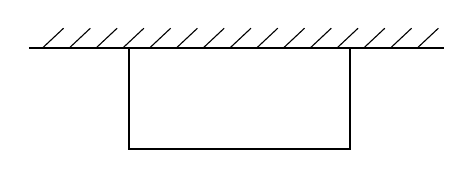
\begin{tikzpicture}[scale=0.85]
  \draw[thick] (-0.7,1.5) -- (5.5,1.5);
  \foreach \x in {-0.5,-0.1,...,5.1}
    \draw (\x,1.5) -- ++(0.32,0.3);
  \draw[thick] (0.8,1.5) -- (0.8,0) -- (4.1,0) -- (4.1,1.5);
\end{tikzpicture}
\end{center}
\nopagebreak[4]
\Needspace{4\baselineskip}
\textbf{解析}

按源卷布局重绘的示意图（墙面在上方，砖墙砌矩形的三面）：
\nopagebreak[4]
\begin{center}% 1977 年江苏徐州市,徐州地区初试卷第 7 题：一边靠墙的矩形猪圈示意图（按源卷第 2 页布局）。
% 斜纹线表示原有墙面，砖墙砌矩形的左、下、右三面，上边落在墙线上。
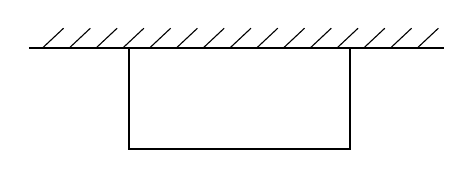
\begin{tikzpicture}[scale=0.85]
  \draw[thick] (-0.7,1.5) -- (5.5,1.5);
  \foreach \x in {-0.5,-0.1,...,5.1}
    \draw (\x,1.5) -- ++(0.32,0.3);
  \draw[thick] (0.8,1.5) -- (0.8,0) -- (4.1,0) -- (4.1,1.5);
\end{tikzpicture}
\end{center}
\nopagebreak[4]
\Needspace{5\baselineskip}
设垂直于墙的一边（宽）为 $x$ 米。靠墙一面不砌，$20$ 米砖墙砌其余三面，故平行于墙的一边长为 $(20-2x)$ 米，且须 $20-2x>0$，即 $0<x<10$。猪圈面积

\nopagebreak[4]
\[
S=x(20-2x)=-2x^2+20x=-2(x-5)^2+50.
\]

当 $x=5$ 时 $S$ 取最大值 $50$，此时平行于墙的一边长为 $10$ 米。即宽取 $5$ 米时猪圈面积最大，最大面积为 $50$ 平方米。

\gkanswer{答案：宽取 $5$ 米（此时长为 $10$ 米），最大面积 $50$ 平方米。}

\end{answer}
\begin{answer}
\gksolhead{8}{}

\textbf{题目}（14 分）：

已知：$\lg2=0.3010$，$\lg3=0.4771$。计算从 $1$ 到 $10$ 之间（除 $7$ 以外）所有整数的对数值。

\Needspace{4\baselineskip}
\textbf{解析}

\Needspace{5\baselineskip}
利用给定值与对数运算律，从 $1$ 到 $10$ 之间（除 $7$ 以外）各整数的对数值为

\nopagebreak[4]
\[
\lg1=0,
\]

\nopagebreak[4]
\[
\lg2=0.3010,\qquad
\lg3=0.4771\ \text{（\text{已知}）},
\]

\nopagebreak[4]
\[
\lg4=2\lg2=0.6020,
\]

\nopagebreak[4]
\[
\lg5=\lg\frac{10}{2}=1-\lg2=0.6990,
\]

\nopagebreak[4]
\[
\lg6=\lg2+\lg3=0.7781,
\]

\nopagebreak[4]
\[
\lg8=3\lg2=0.9030,
\]

\nopagebreak[4]
\[
\lg9=2\lg3=0.9542,
\]

\nopagebreak[4]
\[
\lg10=1.
\]

（$\lg7$ 按题意不要求。）

\gkanswer{答案：$\lg1=0$，$\lg2=0.3010$，$\lg3=0.4771$，$\lg4=0.6020$，$\lg5=0.6990$，$\lg6=0.7781$，$\lg8=0.9030$，$\lg9=0.9542$，$\lg10=1$。}

\end{answer}
\begin{answer}
\gksolhead{9}{}

\textbf{题目}（12 分）：

已知顶点在原点的抛物线，关于 $y$ 轴对称，并且经过 $P(6,-2)$ 点。

（1） 求抛物线的方程；

（2） 画出它的大致图形；

（3） 写出它的焦点坐标和准线方程。

\Needspace{4\baselineskip}
\textbf{解析}

\gksubpart{（1）}

\Needspace{5\baselineskip}
顶点在原点且关于 $y$ 轴对称的抛物线可设为

\nopagebreak[4]
\[
x^2=\pm2py\qquad(p>0).
\]

\Needspace{5\baselineskip}
它经过 $P(6,-2)$，该点纵坐标为负，曲线只能开口向下，故取

\nopagebreak[4]
\[
x^2=-2py.
\]

\Needspace{5\baselineskip}
代入 $P(6,-2)$：

\nopagebreak[4]
\[
36=-2p\times(-2)=4p,
\qquad
p=9.
\]

\Needspace{5\baselineskip}
故抛物线方程为

\nopagebreak[4]
\[
x^2=-18y.
\]

\gksubpart{（2）}

曲线开口向下，顶点在原点，过 $P(6,-2)$，由对称性也过 $(-6,-2)$。大致图形如下：
\nopagebreak[4]
\begin{center}% 1977 年江苏徐州市,徐州地区初试卷第 9 题（2）小问：抛物线 x^2=-18y 的大致图形（编者按题意补绘，非源卷插图）。
\begin{tikzpicture}[scale=0.5]
  \draw[-stealth] (-8,0) -- (8,0) node[below] {$x$};
  \draw[-stealth] (0,-6.5) -- (0,1.8) node[left] {$y$};
  \node[below left] at (0,0) {$O$};
  \draw[thick,domain=-7.4:7.4,samples=41] plot (\x,{-\x*\x/18});
  \fill (6,-2) circle (1.5pt) node[right] {$P(6,\,-2)$};
  \fill (-6,-2) circle (1.5pt) node[left] {$(-6,\,-2)$};
\end{tikzpicture}
\end{center}
\nopagebreak[4]
\gksubpart{（3）}

\Needspace{5\baselineskip}
$p=9$，焦点在 $y$ 轴负半轴，准线在 $y$ 轴正半轴：

\nopagebreak[4]
\[
F\left(0,-\frac{p}{2}\right)=\left(0,-\frac{9}{2}\right),
\qquad
\text{\text{准线：}}\ y=\frac{p}{2}=\frac{9}{2}.
\]

\gkanswer{答案（1）：$x^2=-18y$。}

\gkanswer{答案（2）：见解析版}

\gkanswer{答案（3）：焦点 $\left(0,-\dfrac{9}{2}\right)$，准线 $y=\dfrac{9}{2}$。}

\end{answer}
\begin{answer}
\gksolhead{10}{}

\textbf{题目}（10 分）：

已知：$a$，$15$，$b$ 三个数成等差数列；$a$，$9$，$b$ 三个数成等比数列。求 $a$、$b$ 两个数。

\Needspace{4\baselineskip}
\textbf{解析}

\Needspace{5\baselineskip}
由 $a$，$15$，$b$ 成等差数列，得

\nopagebreak[4]
\[
a+b=2\times15=30.
\]

\Needspace{5\baselineskip}
由 $a$，$9$，$b$ 成等比数列，得

\nopagebreak[4]
\[
9^2=ab,
\qquad
ab=81.
\]

\Needspace{5\baselineskip}
于是 $a$、$b$ 是二次方程

\nopagebreak[4]
\[
t^2-30t+81=0
\]

\Needspace{5\baselineskip}
的两根。由 $(t-3)(t-27)=0$ 得 $t=3$ 或 $t=27$，因此

\nopagebreak[4]
\[
(a,b)=(3,27)\ \text{\text{或}}\ (27,3).
\]

两组均满足题设：$3,15,27$ 与 $27,15,3$ 都是等差数列，$3,9,27$ 与 $27,9,3$ 都是等比数列。故 $a=3$，$b=27$；或 $a=27$，$b=3$。

\gkanswer{答案：$a=3$，$b=27$；或 $a=27$，$b=3$。}

\end{answer}